\chapter{Tests}
Experiments were conducted using the provided test program and complementary testing was performed with \textit{Apache Benchmark} as this is often used to test performance of HTTP servers. During the testing the server had a artificial load of 40 ms to perform each request. The load came from a sleep statement in the process method which means that the CPU was not loaded as much as it could have been in a real scenario.

The initial testing was performed to find the best approach to the threading problem. The different versions of the server and with different settings was compared to each other by running the same benchmark sequence in all configurations. In this test, each concurrent process (in the benchmark tool) tried to perform 10 requests. The result is illustrated in figure \ref{fig:performance-compare}.

\begin{figure}[h]
\centering
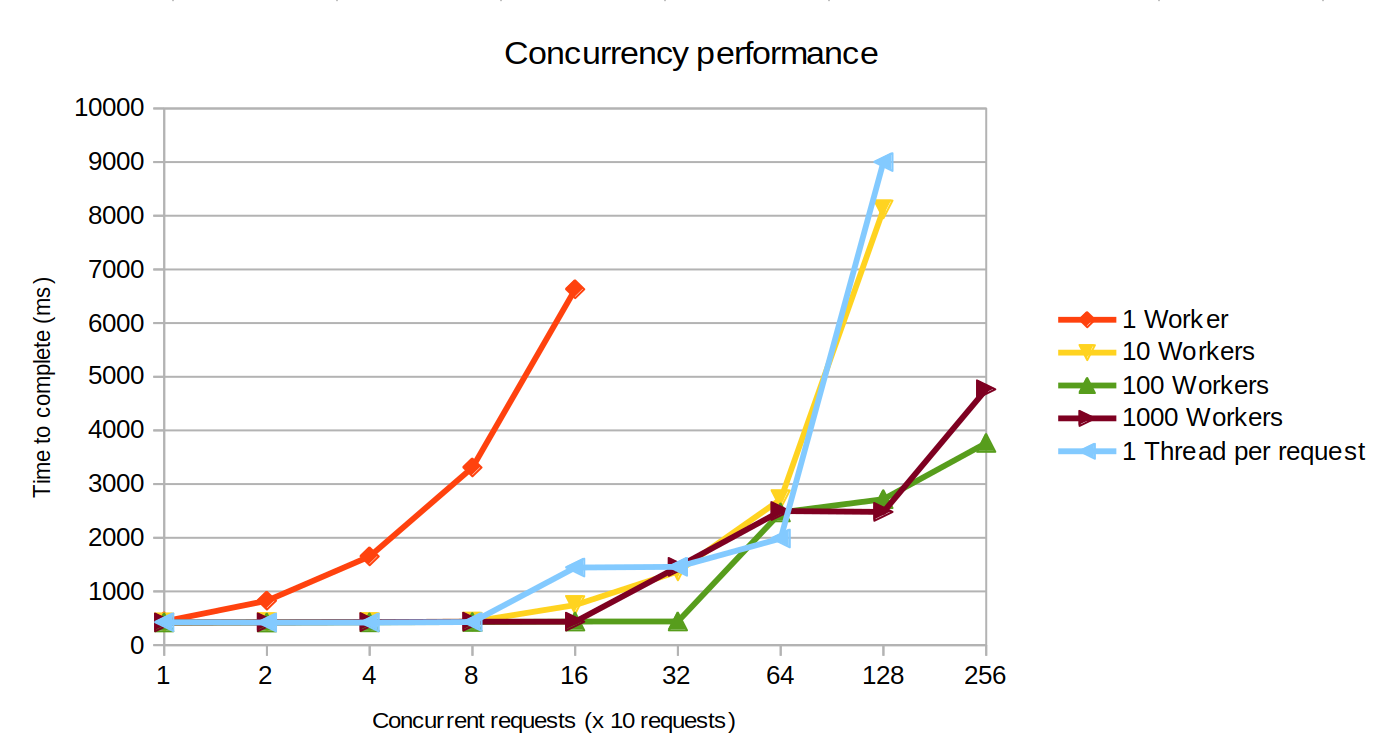
\includegraphics[width=0.87\linewidth]{res/performance-compare}
\caption[Comparison between different threading approaches]{}
\label{fig:performance-compare}
\end{figure}

From this figure we can clearly see that a non-concurrent approach is unusable and some other technique is needed (see red line). The other approaches seemed to scale quite well for some time but then suddenly started to spike in execution time. At a first glance this seemed to be when the server got more concurrent requests than it could handle simultaneously. When looking closer we can see that this effect also appeared in the solution using the "1 request"-"1 process" which clearly does not have such a low limitation in the number of concurrent requests it could process.

The best performer in this test was the solution with 100 concurrent workers which scaled well up to around 256 concurrent requests. After this point the same type of problems as can be seen for the \textit{10 workers} and \textit{1 request-1 process} appear and the time rose to unusable levels. This leads me to believe that this is a operating system/hardware limitation in the number of concurrent connection that my computer can handle. In tests with Apache Benchmark this phenomenon instead showed up as a few connection timing out and increasing the average process time a lot.

When performing the same tests on a newer computer the problem with connections timing out also seemed to be smaller but still existing. This further strengthens the statement that this could because of hardware/operating system limitation.

When running apache benchmark with a total of 4000 requests and 1000 simultaneously connected clients (using 100 workers on the server) we get the following result.

\begin{lstlisting}
Time taken for tests:   1.783 seconds
Failed requests:        0
Time per request:       0.446 [ms] (mean)
\end{lstlisting}

This means that we can serve approximately 135'000 requests each minute if we expect that the number of concurrent clients are 1000. This is a relatively high number for a initial attempt at a web server without any caching mechanics and is sufficient for most simple use cases.



